\chapter{\bbbar-tagging of AK8 Jets}
\label{chap:bb}

A novel approach has been studied to identify large-radius jets composed of two b quarks \cite{CMS-PAS-BTV-15-002}. A dedicated multivariate (MVA) tagging algorithm is implemented to combine the information from secondary vertices, tracks, and subjet axes to optimize the discrimination between jets containing two b quarks and those containing a single parton. Input variables which do not depend on the momentum or mass of the parent are chosen to allow consistent performance over a wide range. Tracks with $p_{T}>1\,\textrm{GeV}$ are associated to a jet if they are within a cone of $\Delta R<0.8$ around the jet. A track is associated with a subjet if its distance of closest approach with the subjet axis is less than $700\,\mu\mathrm{m}$ and if its distance of closest approach with the primary vertex is less than $5\,\mathrm{cm}$. The impact parameter significance with respect to the primary vertex is used to discriminate tracks from b decay with prompt tracks. Several input variables make use of the secondary vertices that are reconstructed using the Inclusive Vertex Finder~\cite{CMS-PAS-BTV-15-001}, which identifies secondary vertices independently of the jet clustering. The list of final input variables to the MVA discriminant are detailed in ~\cite{CMS-PAS-BTV-15-002}.  Figure~\ref{fig:DoubleBROCBHadrons} shows the discrimination between between signal $H\rightarrow b\overline{b}$ and background jets based on the true number of b-hadrons.

\begin{figure}
  \begin{center}
    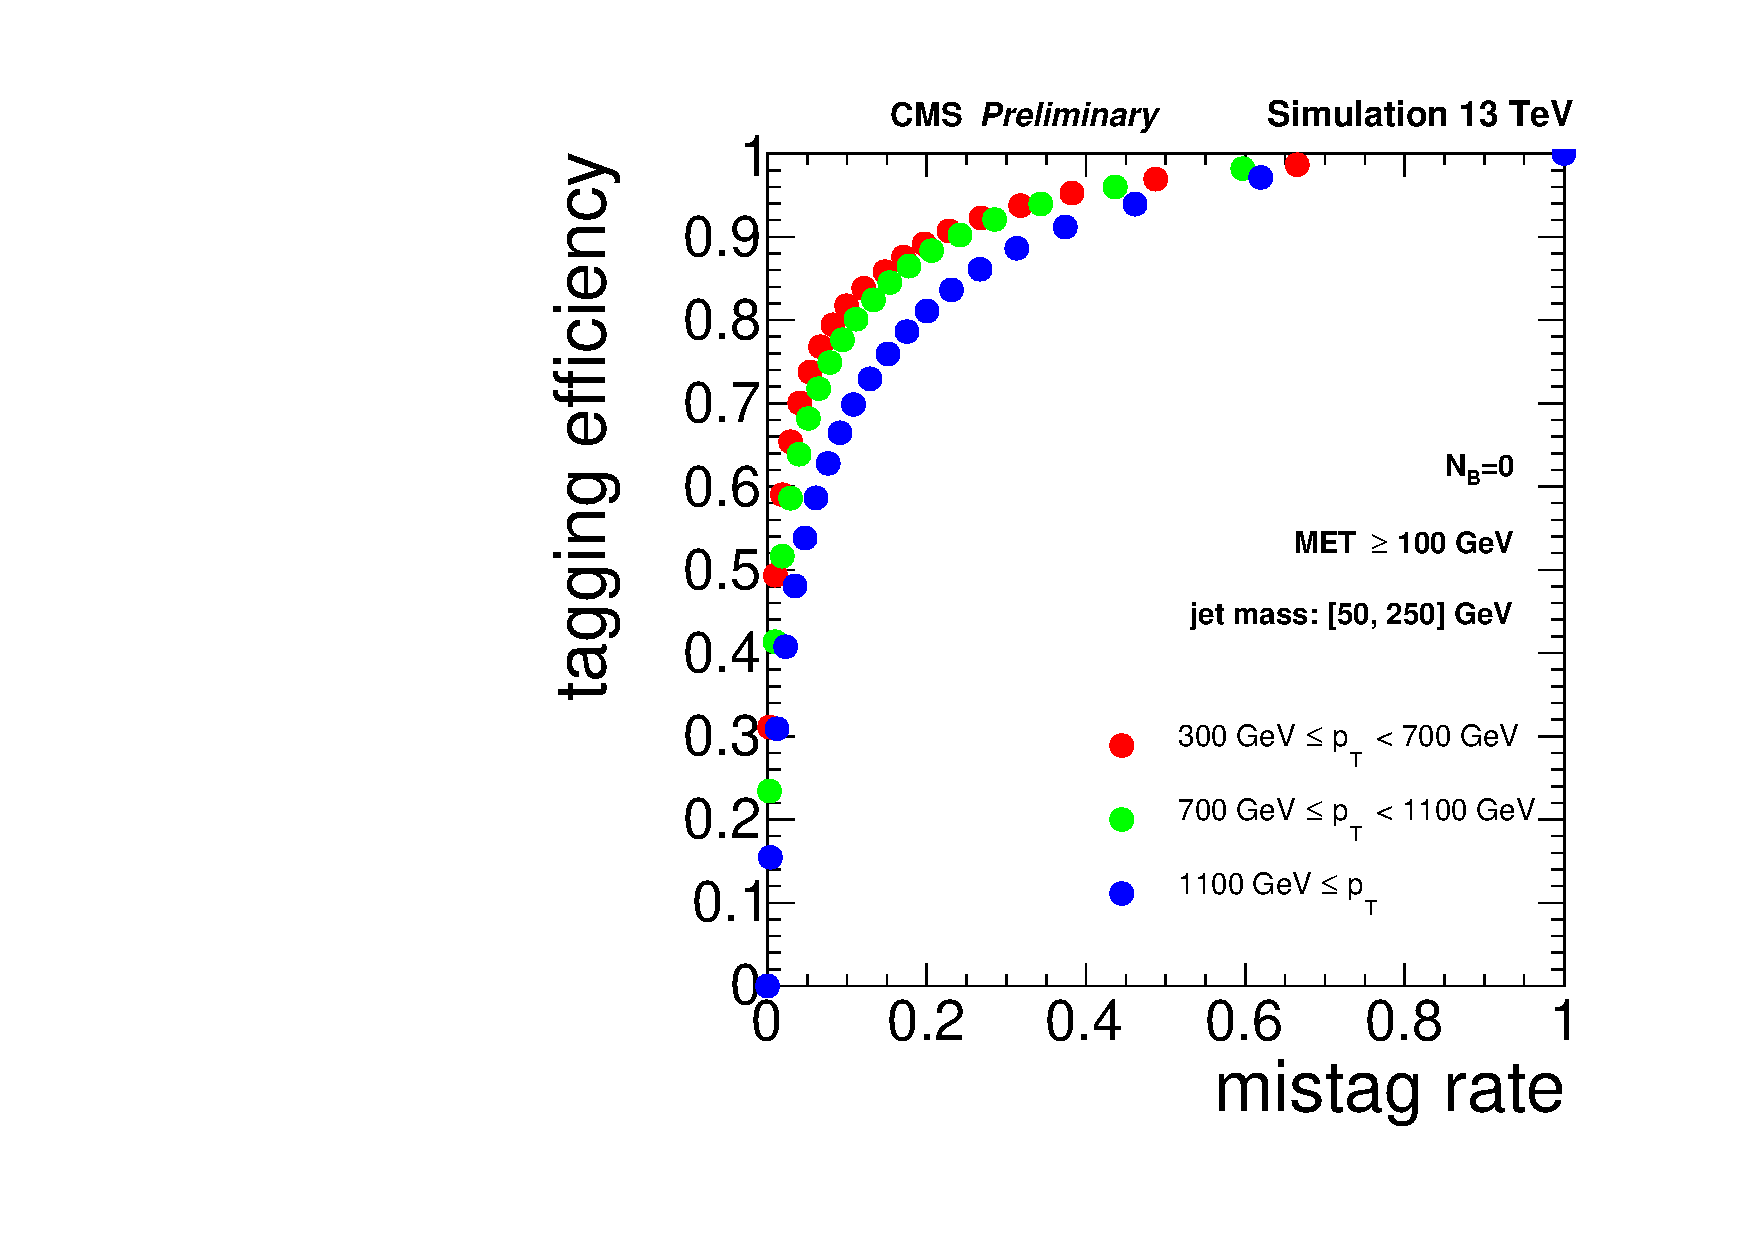
\includegraphics[width=0.32\linewidth]{figs/roc0b.pdf} 
    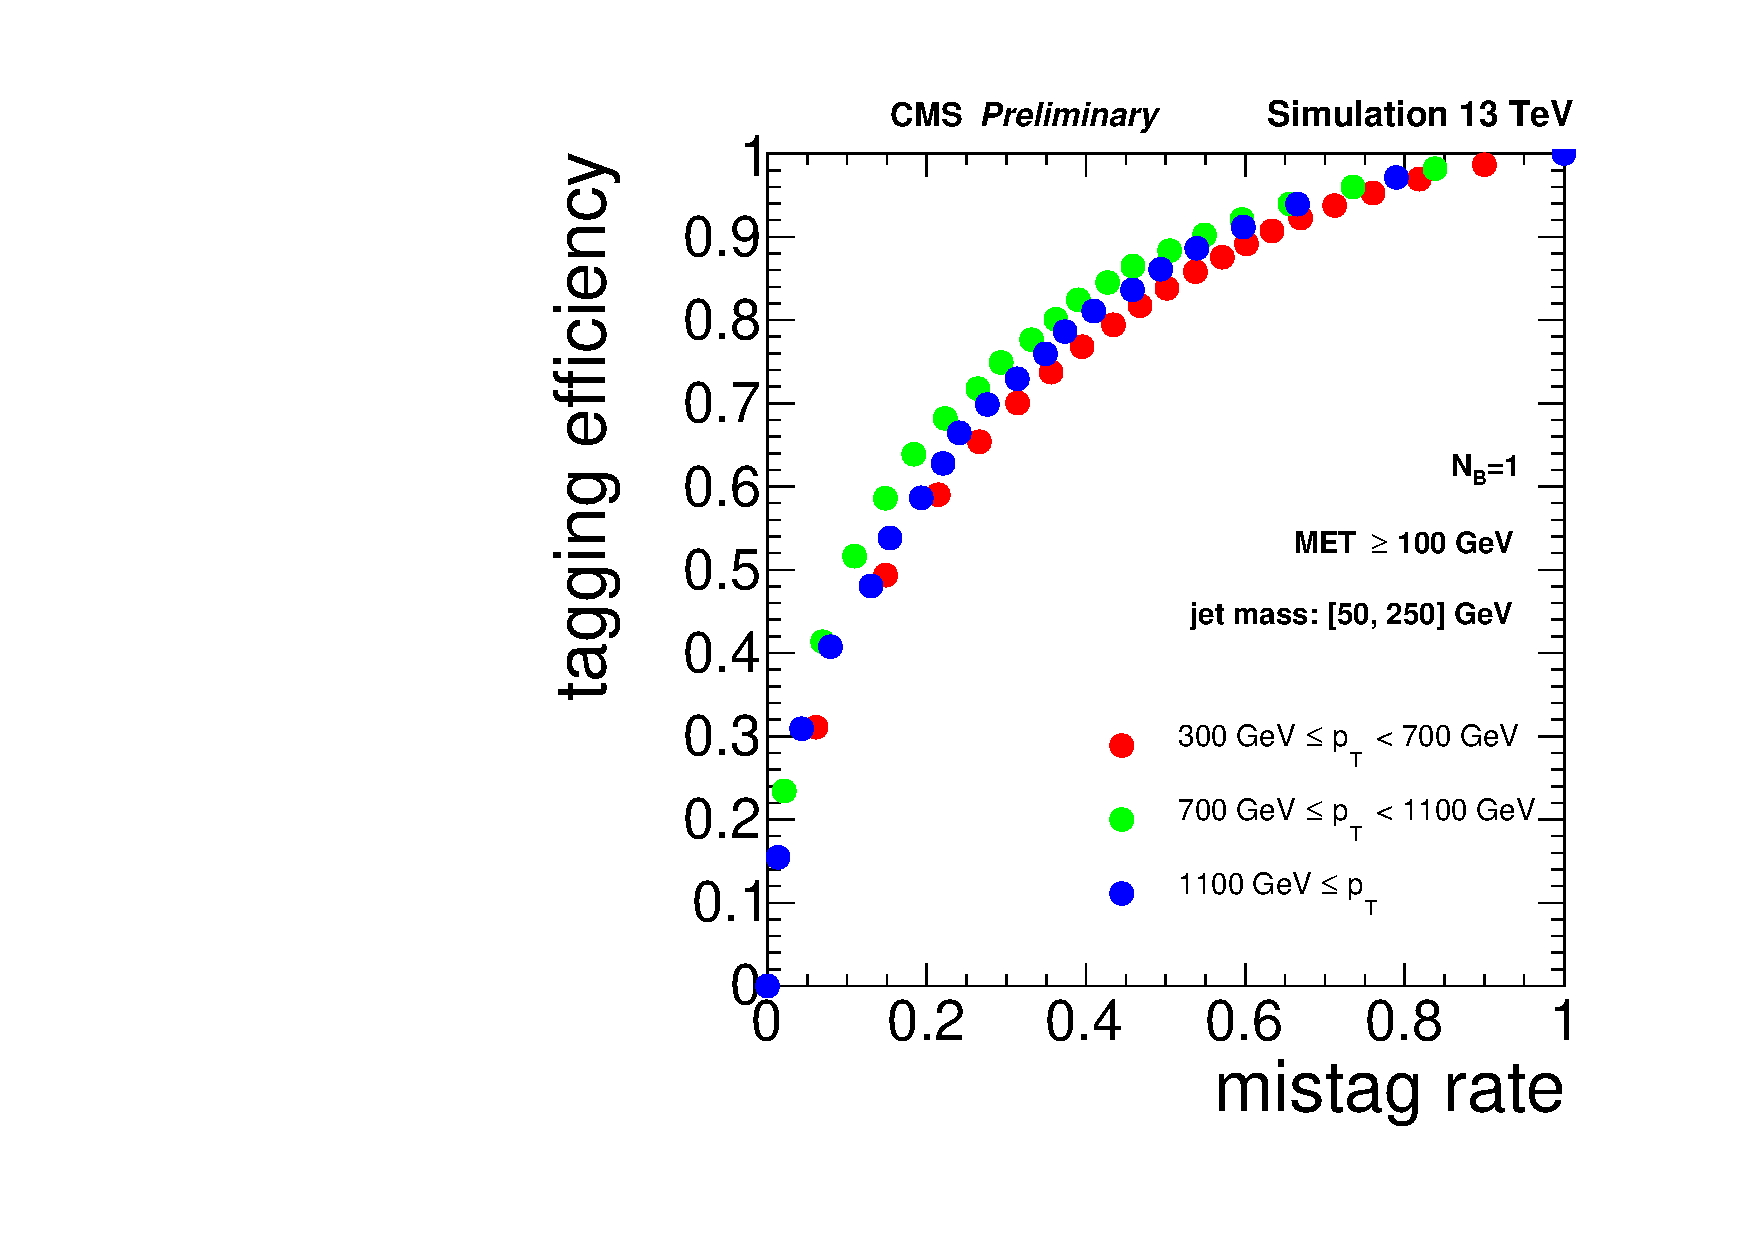
\includegraphics[width=0.32\linewidth]{figs/roc1b.pdf}
    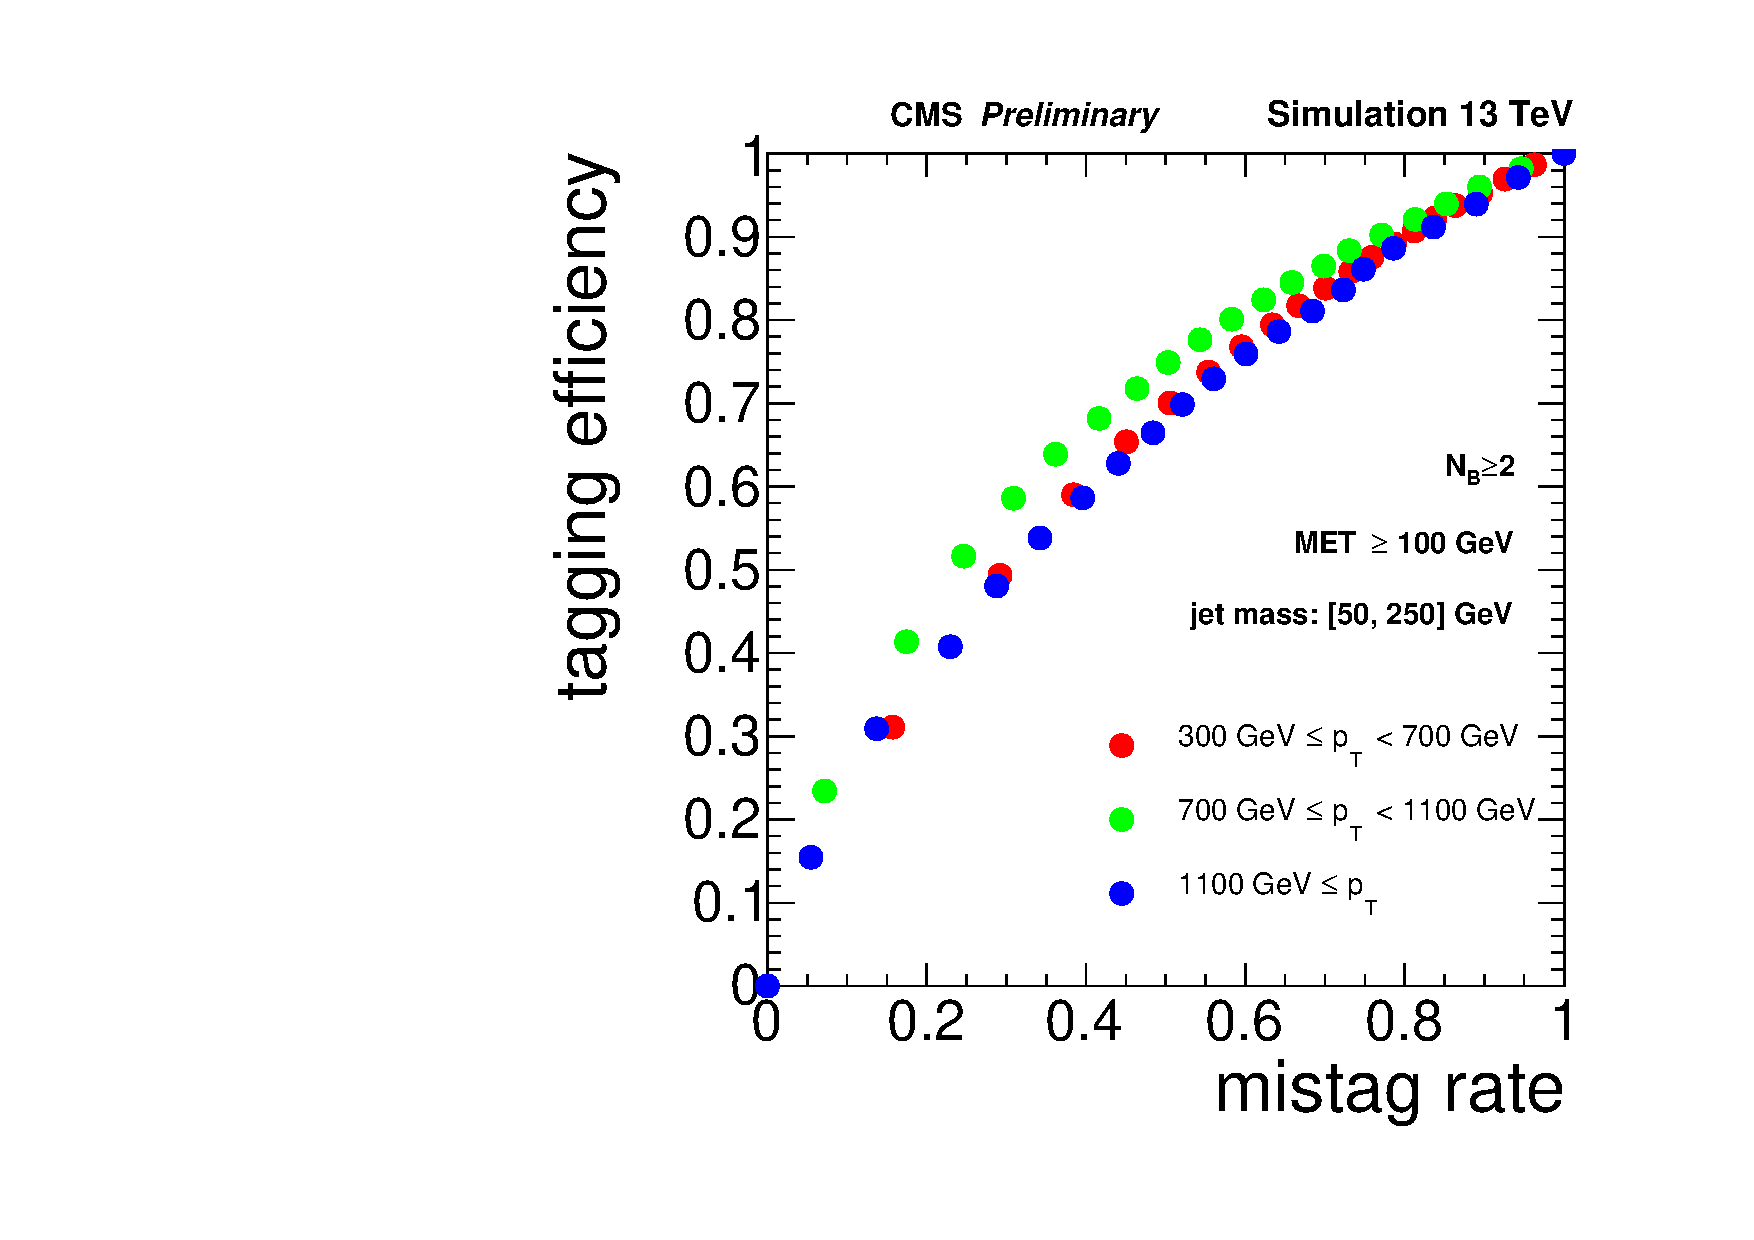
\includegraphics[width=0.32\linewidth]{figs/roc2b.pdf}
\caption
[ROC curve of the signal efficiency and mistag rate for the \bbbar tagger. ]
{ROC curve of the signal efficiency and mistag rate for the \bbbar tagger. The mistag rate is calculated using all expected SM backgrounds.}
    \label{fig:DoubleBROCBHadrons}
  \end{center}
\end{figure}

The central and right plots of Figure~\ref{fig:DoubleBEff} show the signal efficiency for a $H\rightarrow b\bar{b}$ jet to pass the Double-b tag cut for the [85, 135 GeV] and [50, 250 GeV] mass windows, respectively. The efficiencies are computed by matching reconstructed jets to a generator-level Higgs or Z boson based on an angular requirement, $\Delta R<0.8$, between the jet and the appropriate generated particle. Additionally, the reconstructed jet is required to have one or more generated b-hadrons associated with it (jet.jetFlavourInfo().getbHadrons().size()). The efficiency is above $80\%$ for the Double-b discriminator alone, and drops to $~65\%$ when the pruned mass cut is applied. At high jet \pt there is an inefficiency in the double-b tag as tracks from the b quarks become more collimated. The QCD background consists of some mistagged light flavor jets and jets with true b-hadrons that can come from gluon splitting or flavor excitation. The \ttbar background has both true heavy flavor jets and true \ptmiss, but a good number of the single b-hadron jets can be rejected with the Double-b tag requirement.

\begin{figure}
\begin{center}
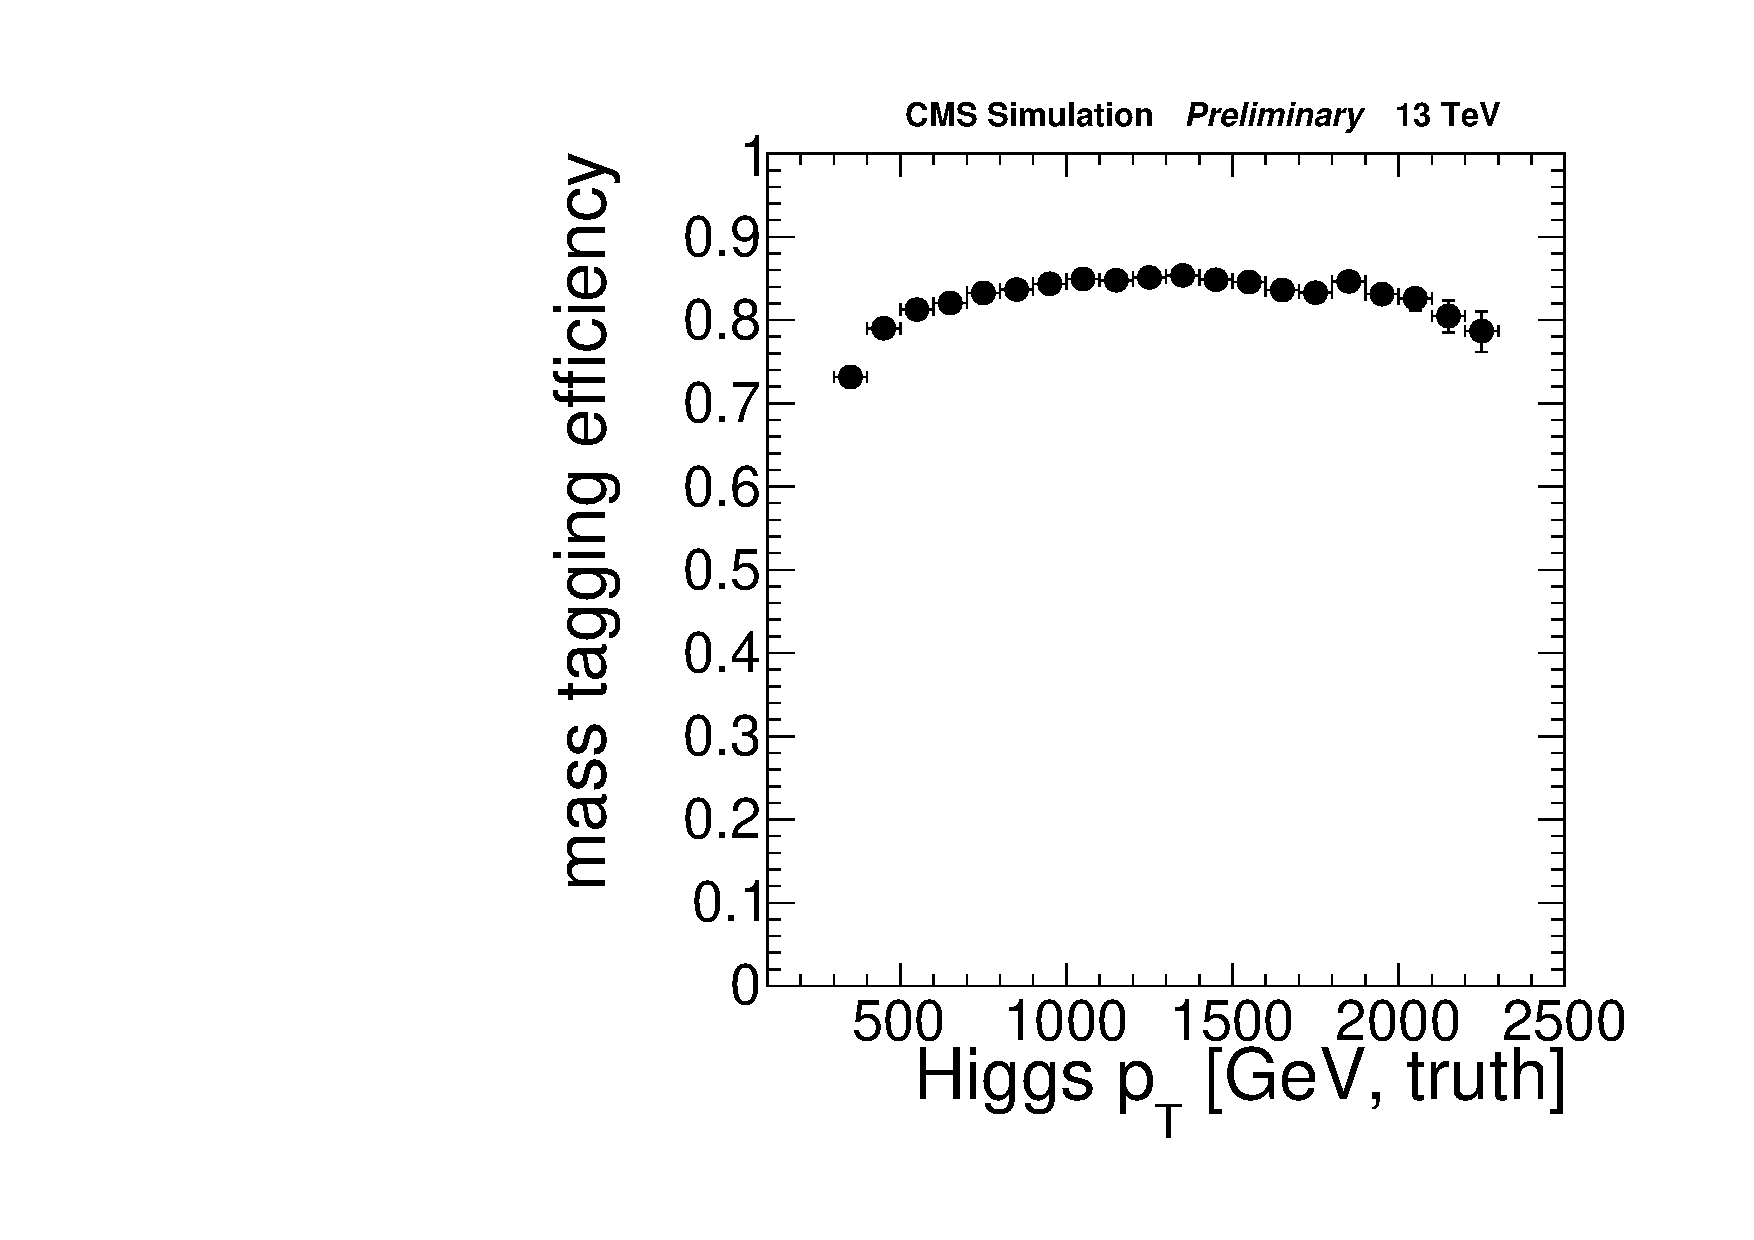
\includegraphics[width=0.32\linewidth]{figs/ptBinnedMassEff.pdf} 
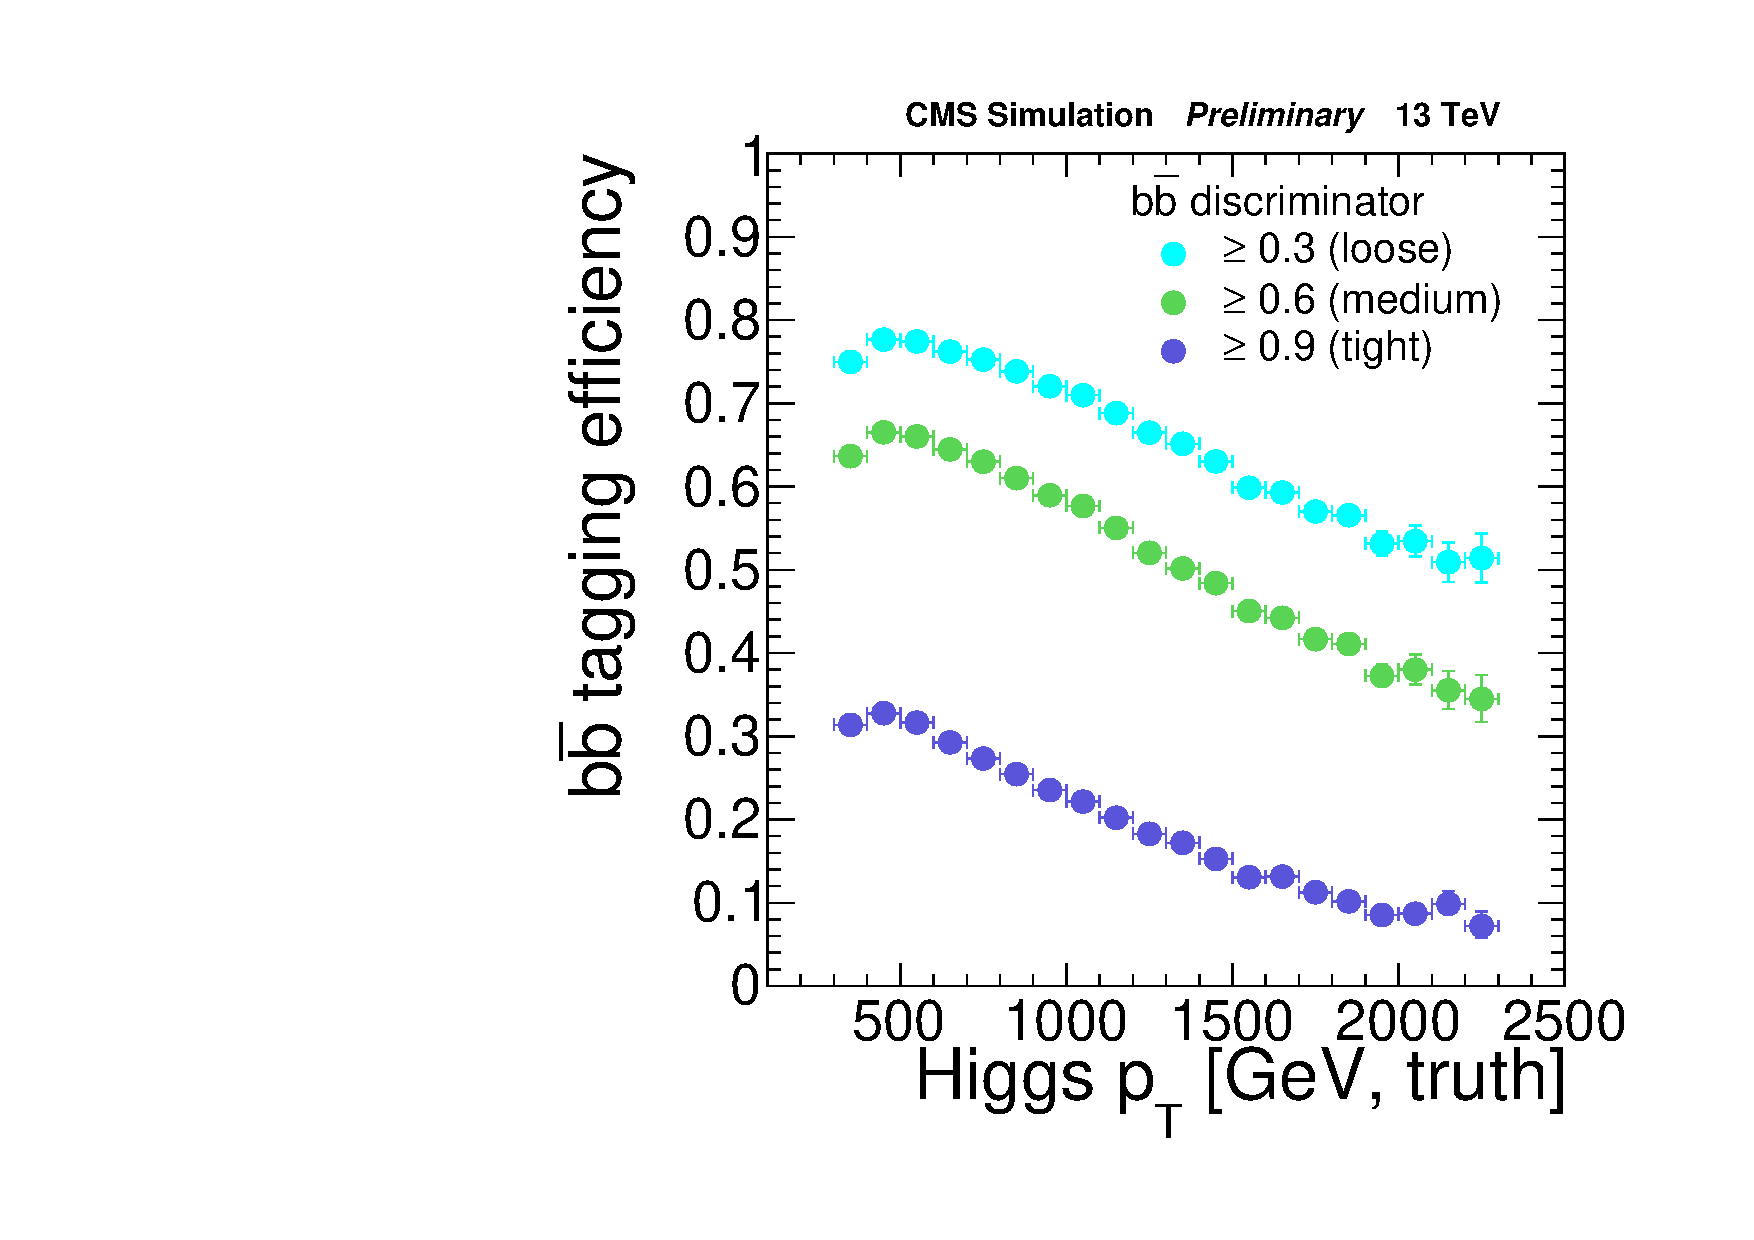
\includegraphics[width=0.32\linewidth]{figs/doubleBEffH.pdf} 
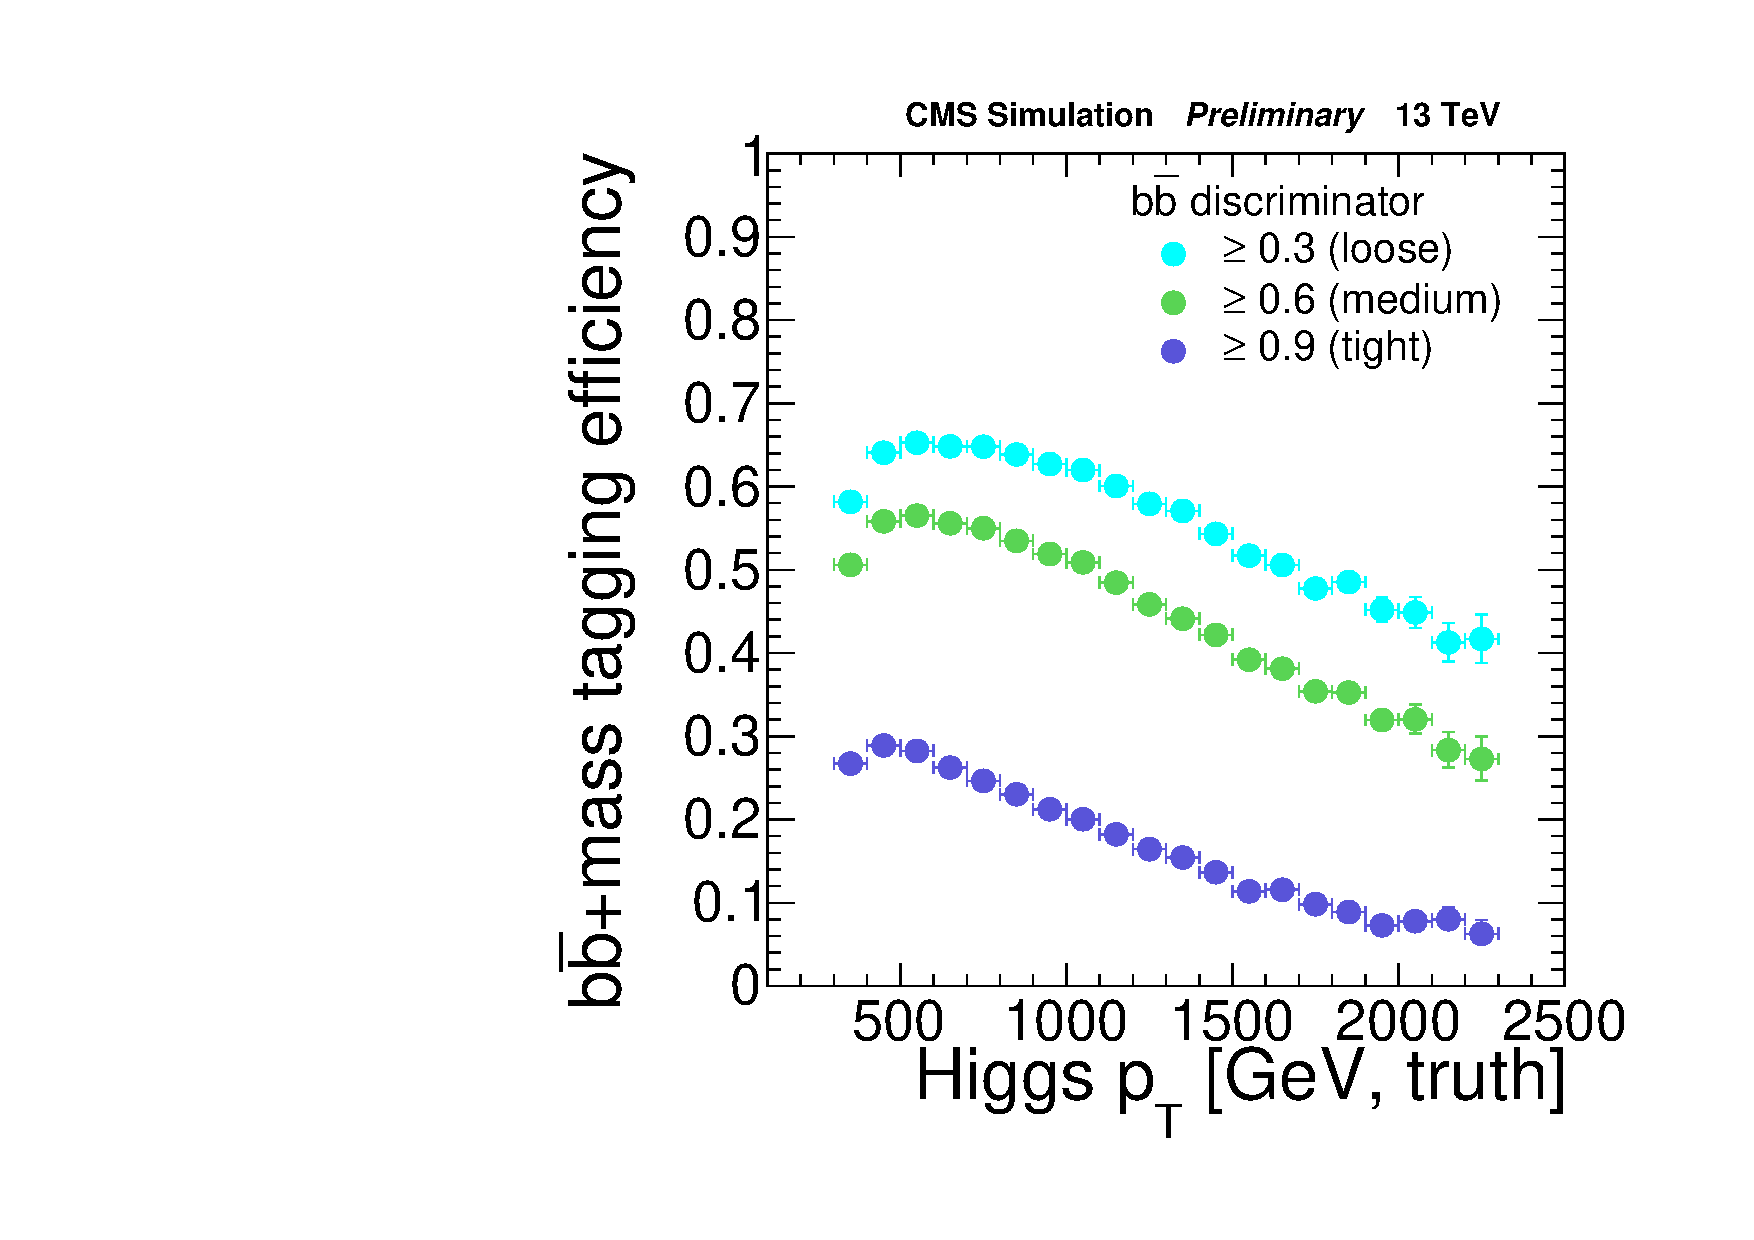
\includegraphics[width=0.32\linewidth]{figs/doubleBEffMassWindowHmass.pdf}
\caption
[$H\rightarrow b\bar{b}$ tagging efficiencies in signal events.]
{The efficiency of a $H\rightarrow b\bar{b}$ jet to have mass [85, 135 GeV], as a function of the generator-level \pt (left). The efficiency of a $H\rightarrow b\bar{b}$ jet to pass the double-b tagging requirement, for three different working points (center). The efficiency of a $H\rightarrow b\bar{b}$ jet to pass both the tight mass and double-b tagging requirements (right).}
\label{fig:DoubleBEff}
\end{center}
\end{figure}

Figure~\ref{fig:HSignalEff} shows the signal efficiency for $H(b\bar{b})H(b\bar{b})$ and $H(b\bar{b})Z(q\bar{q})$ signal models as a function of the double-b discriminator value. For the model with $H(b\bar{b})H(b\bar{b})$, the efficiency is plotted against the smaller of the double-b discriminators of the leading and sub-leading jet, since both are expected to have two b-quarks. For the model with $H(b\bar{b})Z(q\bar{q})$, only one jet is expected to have two b-quarks, so the efficiency is plotted against the larger double-b discriminator value between the leading and sub-leading jet. We use the loose working point of the double-b cut at 0.3 to consider a jet to be double tagged. 

\begin{figure}
\centering
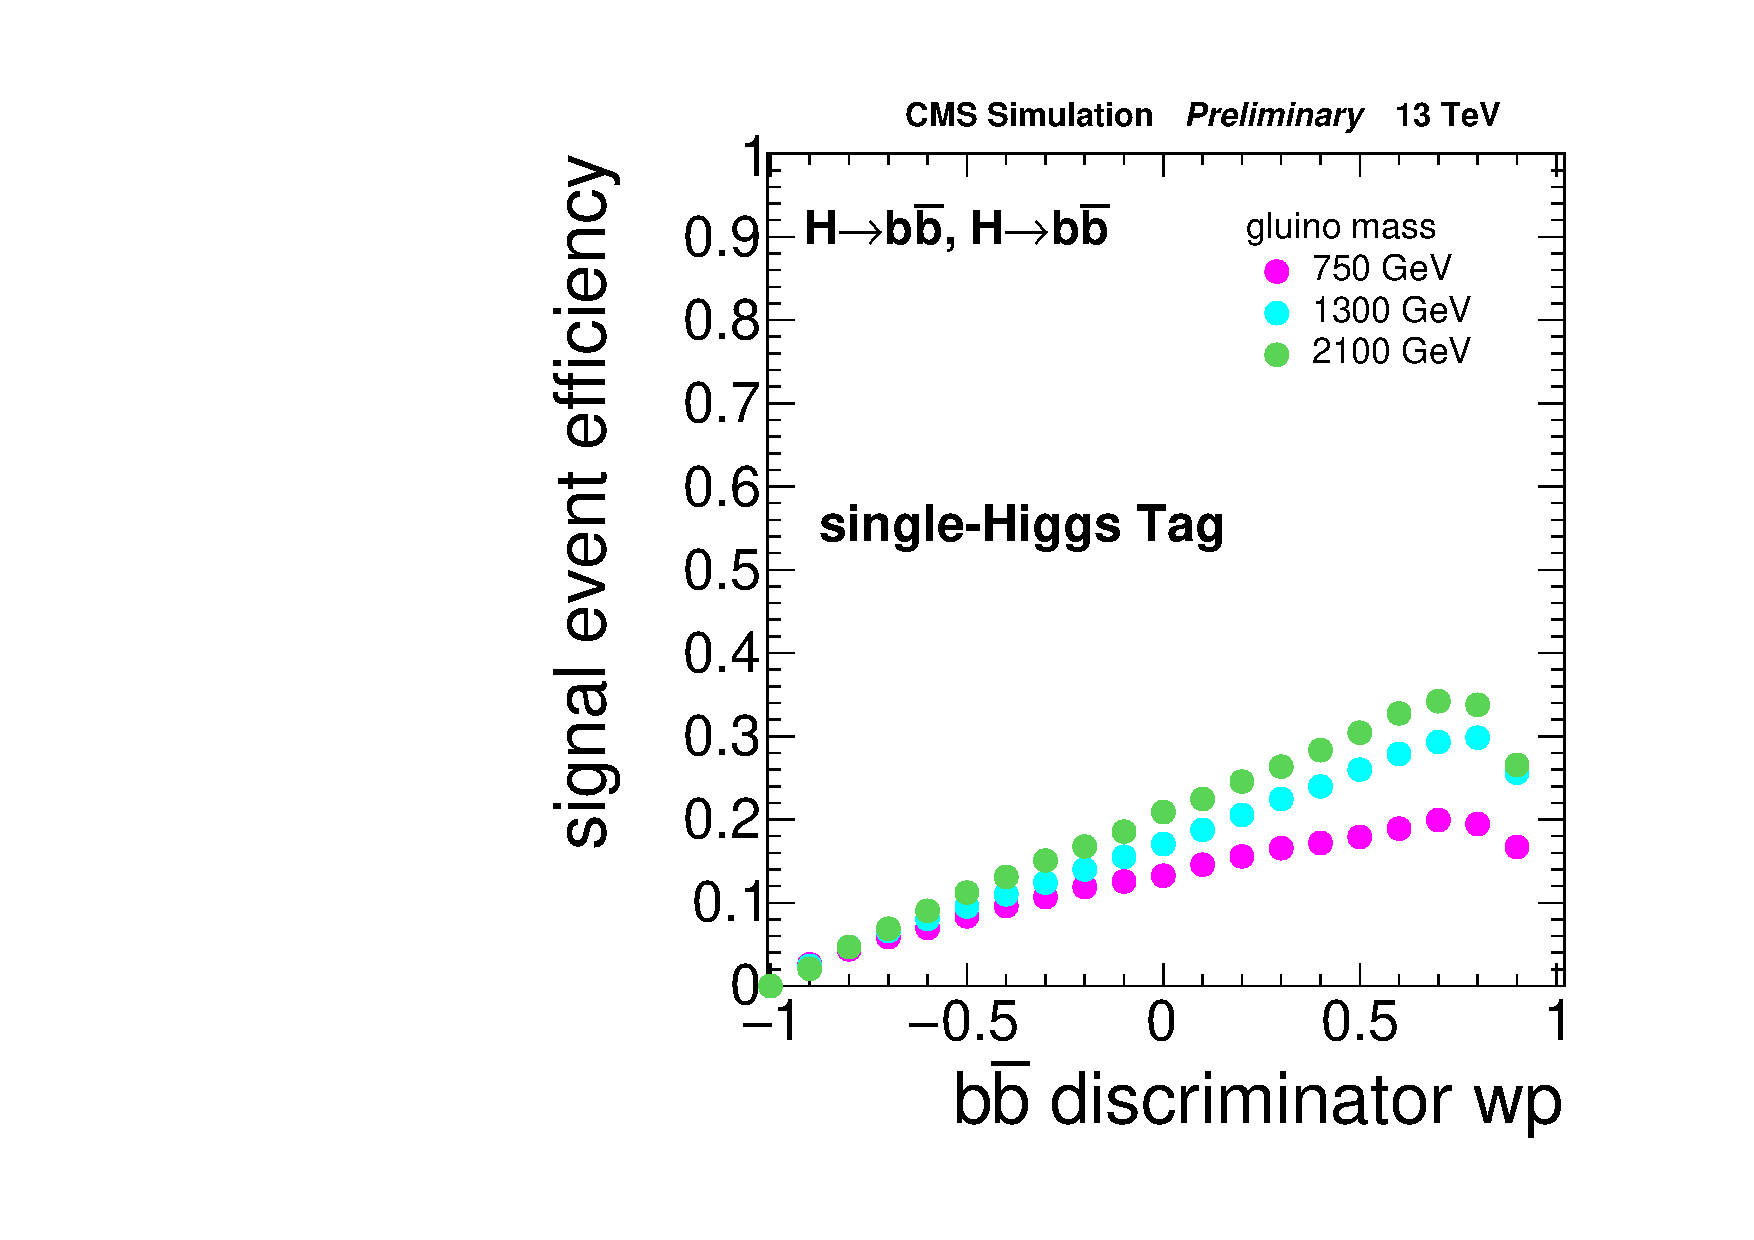
\includegraphics[width=0.32\linewidth]{figs/SingleHiggsTagHH.pdf}
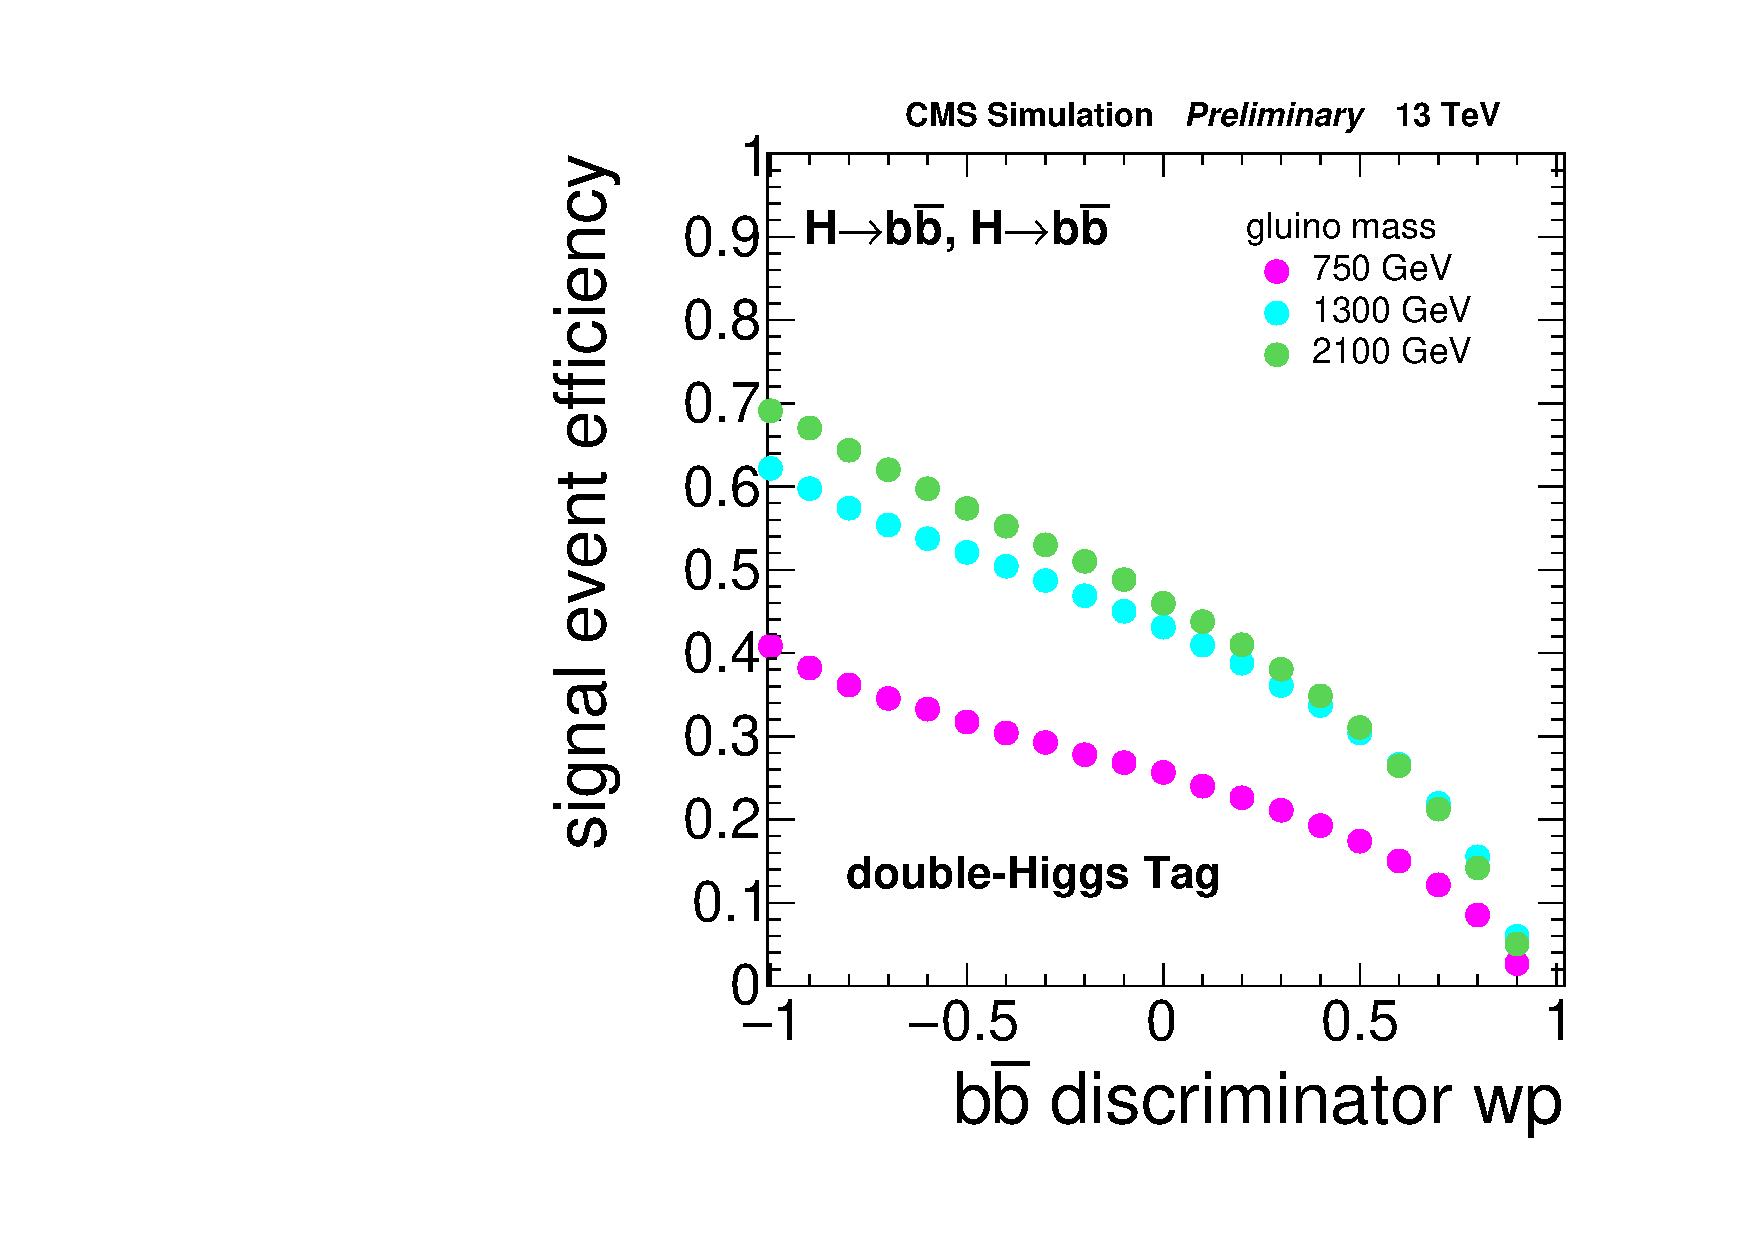
\includegraphics[width=0.32\linewidth]{figs/DoubleHiggsTagHH.pdf}
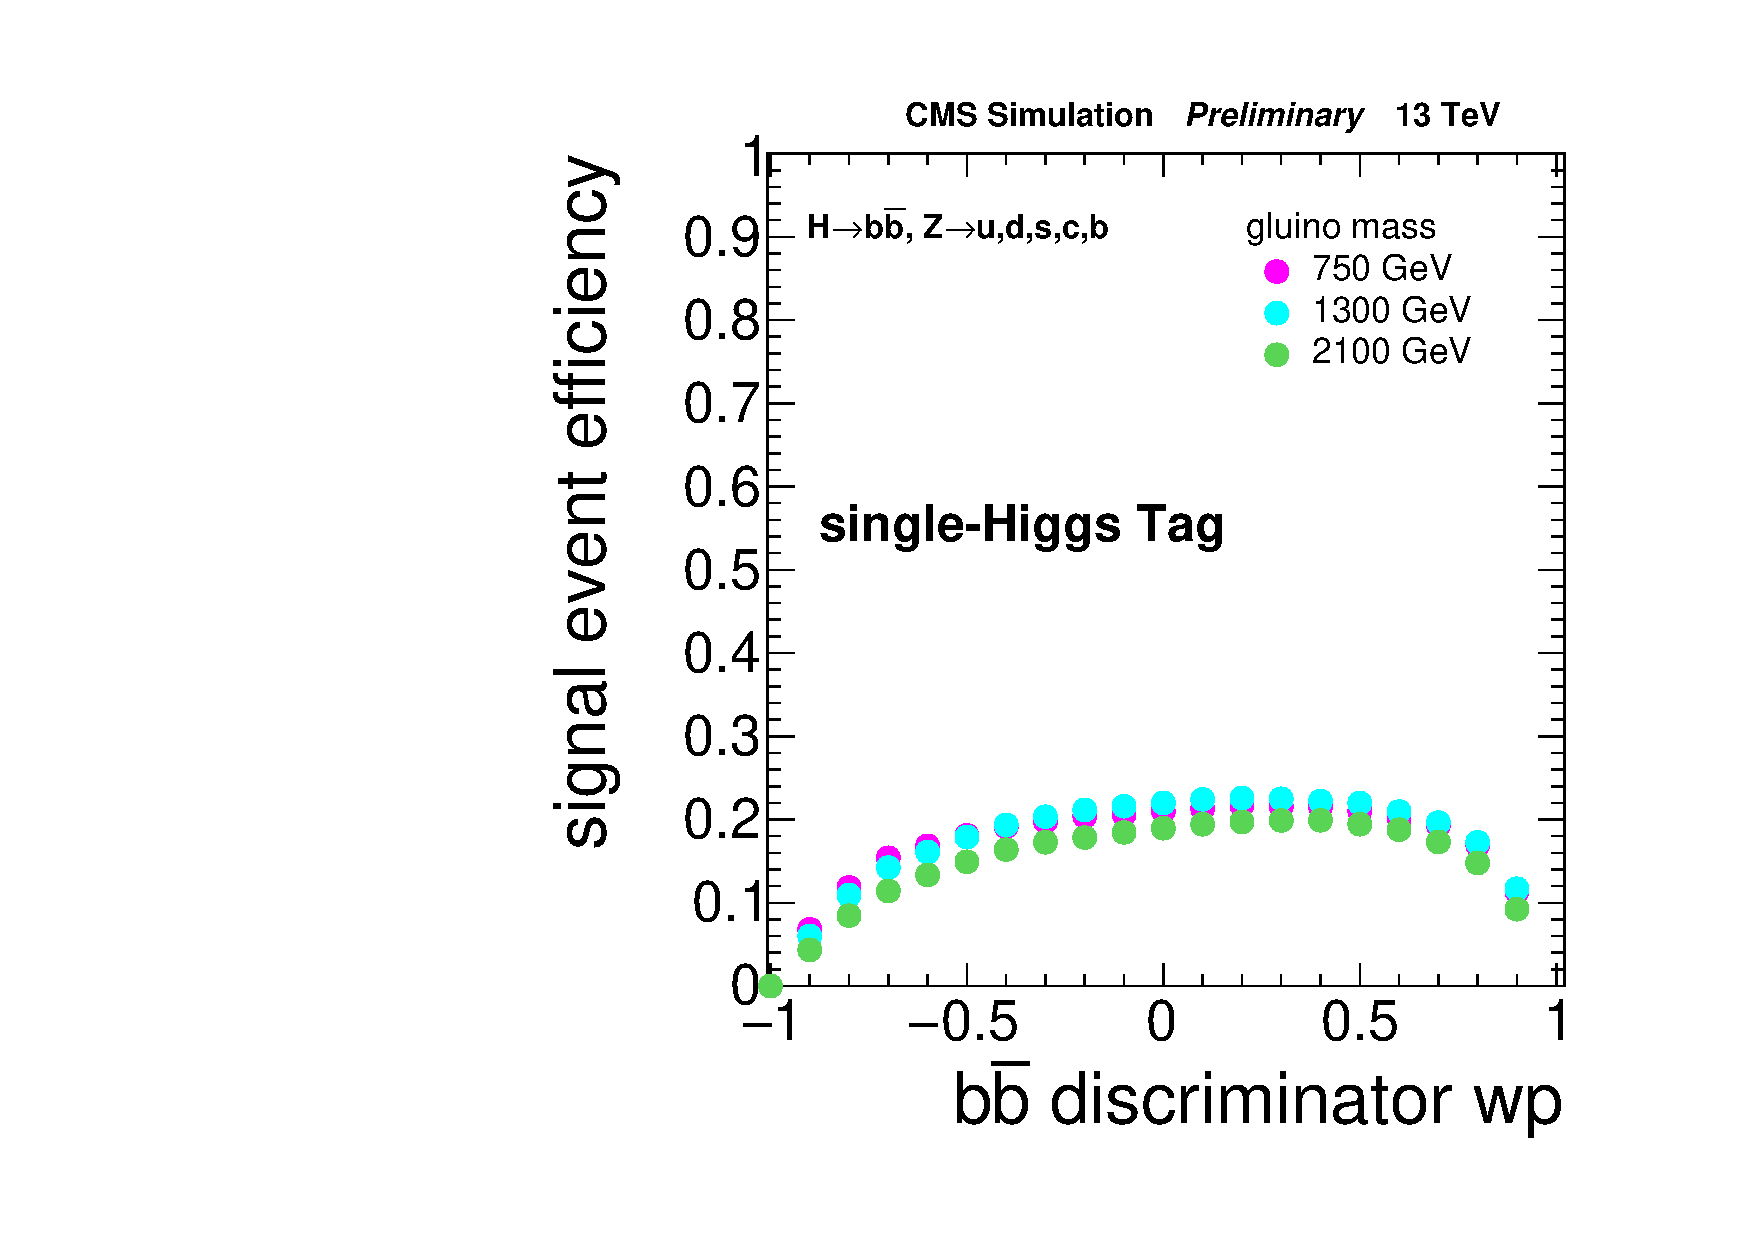
\includegraphics[width=0.32\linewidth]{figs/SingleHiggsTagZH.pdf} 
\caption
[Signal efficiency to be in the single or double Higgs tag event category.]
{Signal efficiency to be in the single or double Higgs tag event category, as a function of the double-b discriminator working-point. Efficiencies are relative to baseline selection. The left and center plots show the single and double Higgs tag efficiencies for the Higgs($b\bar{b}$)-Higgs($b\bar{b}$) MC. The right plot shows the single Higgs tag efficiency for the Z($q\bar{q}$)-Higgs($b\bar{b}$) MC. The curves for three representative gluino masses are shown here.
}
\label{fig:HSignalEff}
\end{figure}


%Figure~\ref{fig:HSignalEff}  shows the signal efficiency for double-b discriminator for the two models. The model with two $H\ri $ decays shows the efficiency vs. the minimum double-b discriminator of the leading and sub-leading jets. 
%Fig.~\ref{fig:DoubleBROCBkgs} shows the discrimination for two background components QCD and in \ttbar. 

%% The two signal models described in Sec~\ref{sec:event-samples} are targetted by defining a single Higgs tag and a two Higgs tag.  The single Higgs region requires both jets to be within the mass window of $\left[85,135\right]\gev$ but only one of them to be Double-b tagged. This allows to capture the Z decays to light flavor quarks in the T5HZ SMS model. For the two Higgs tag region, both jets are in the mass window $\left[85,135\right]\gev$ and both are double-b tagged. These signal regions are designed to supress as much of the background as possible while preserving efficiency for the T5ZH and T5HH signal models. Figure~\ref{fig:HSignalEff} shows the signal efficiency for each signal point vs. the Double-b discriminator.  


%\begin{figure}[htbp!]
%  \begin{center}
%    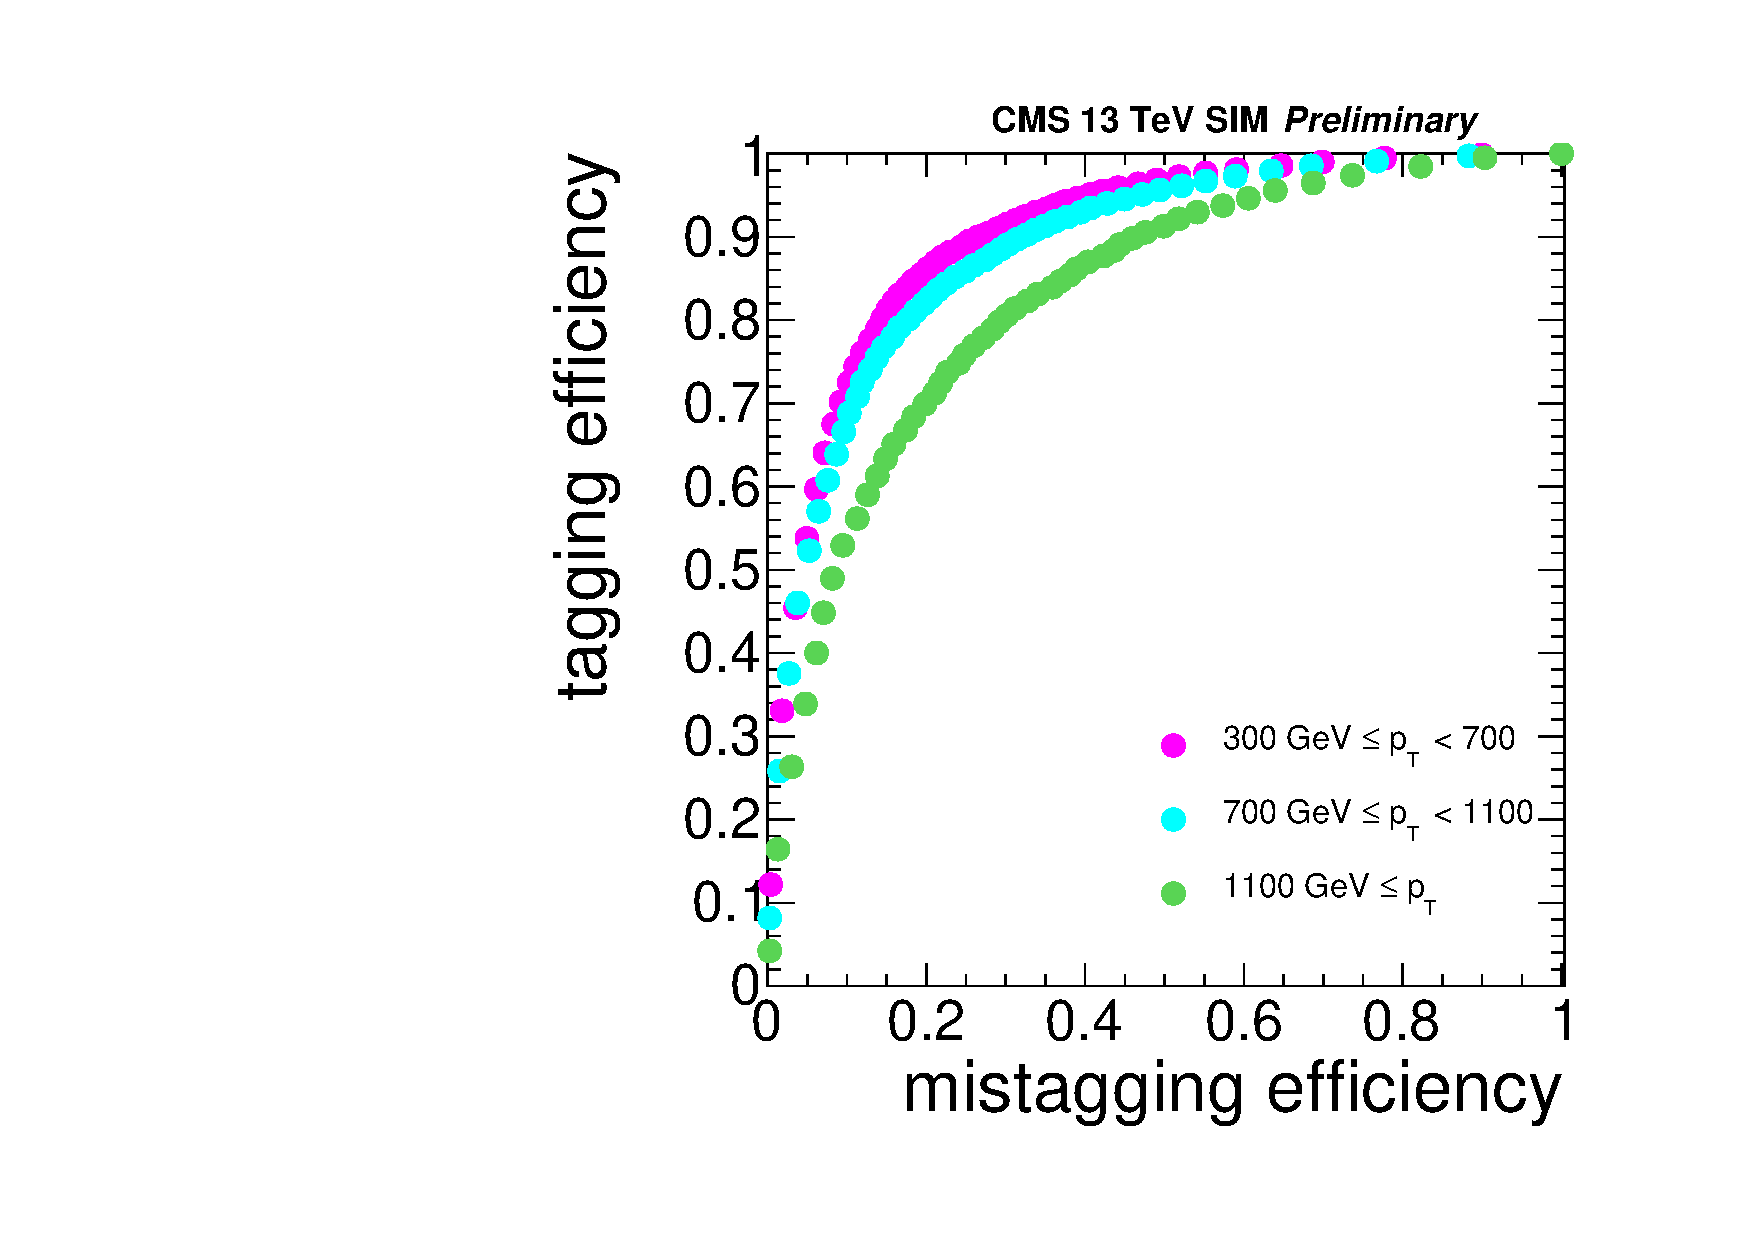
\includegraphics[width=0.48\linewidth]{plots/event-selection/rocHiggsqcd.pdf} 
%    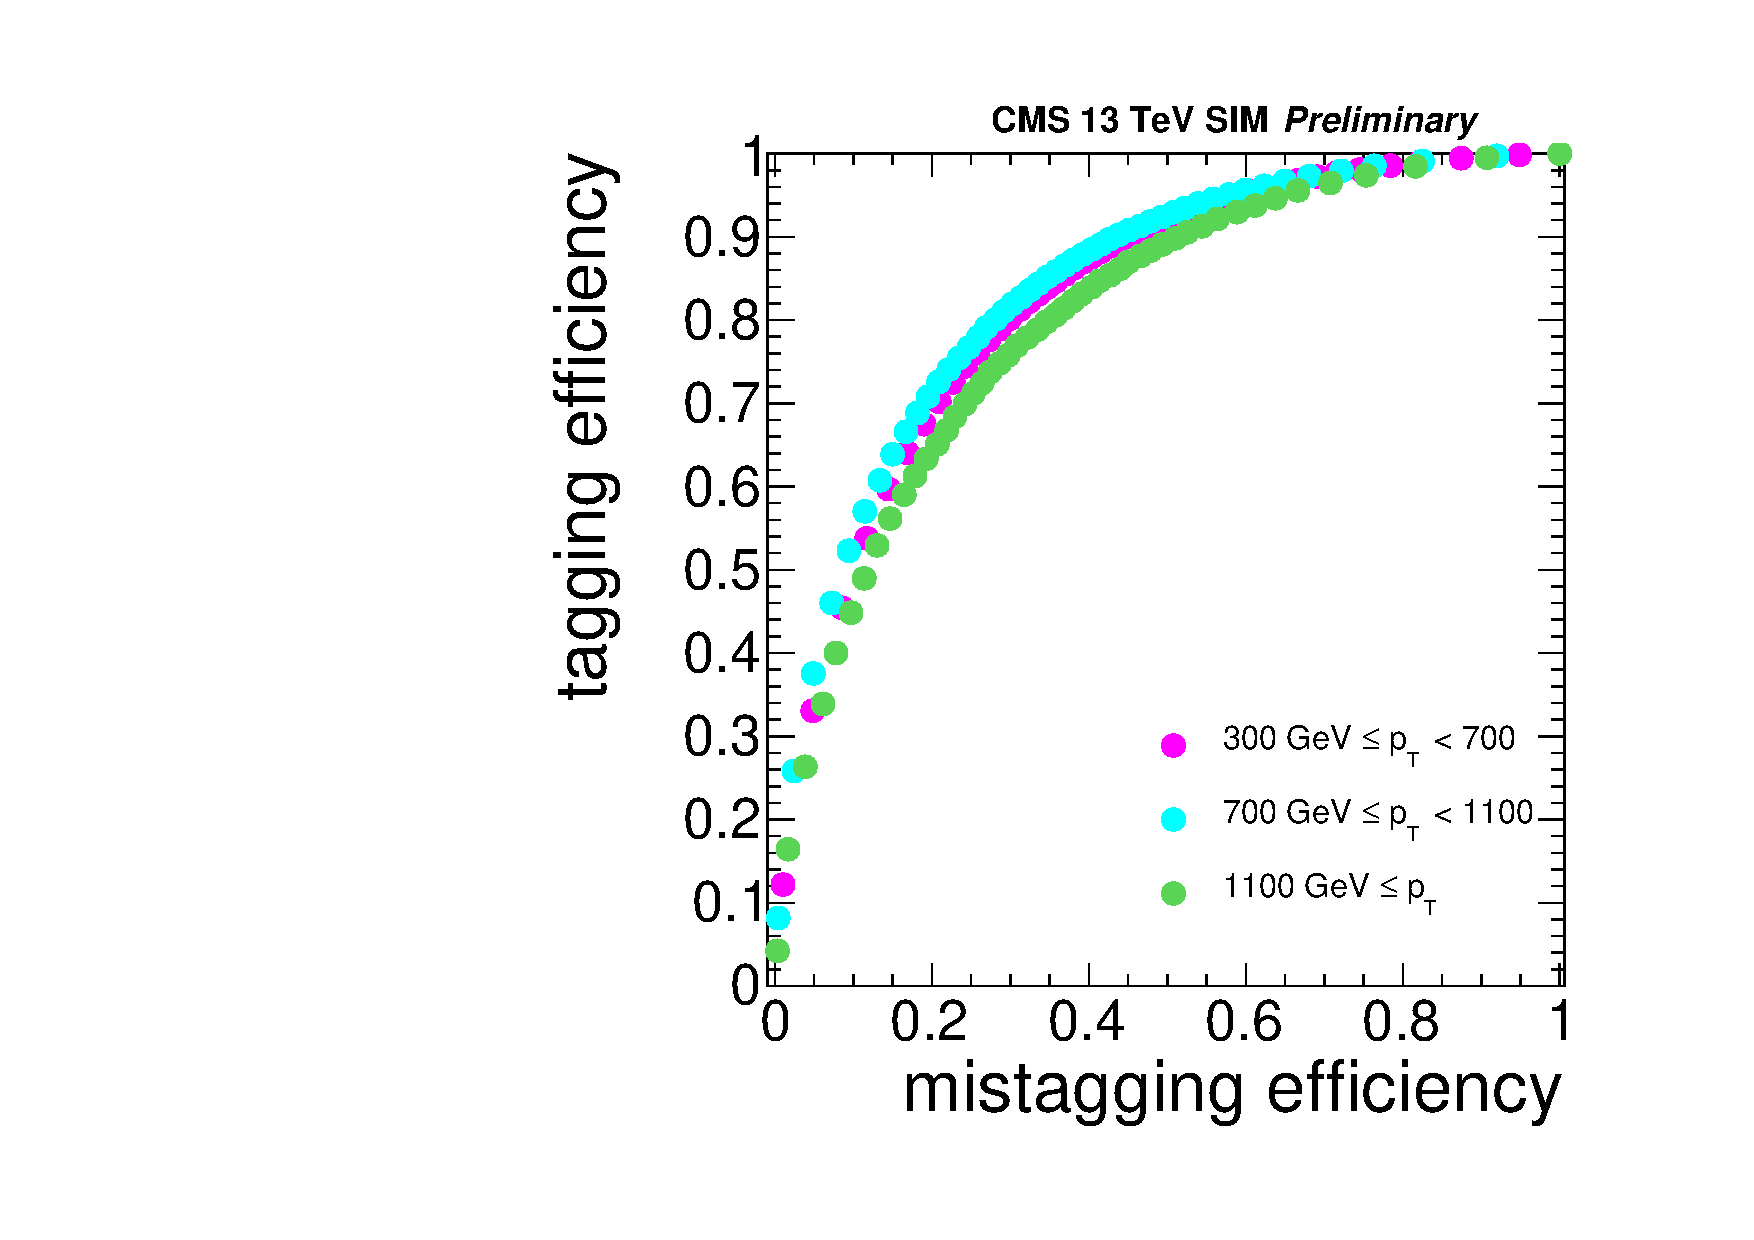
\includegraphics[width=0.48\linewidth]{plots/event-selection/rocHiggsttjets.pdf}
%    \caption{
%	The double-b tagger tag vs mis-tag efficiency is shown for jets in QCD (left) and in \ttbar (right).
%    }
%    \label{fig:DoubleBROCBkgs}
%  \end{center}
%\end{figure}

The efficiency of the double-b tagger is measured in a data sample consisting of high \pt jets enriched in $b\overline{b}$ 
from gluon-splitting. To select a boosted topology similar to the signal, the AK8 jet \pt is required to be above 300 GeV and 
the AK8 pruned mass is required to be above 50 GeV. The jet must also be matched to at least two muons with \pt$>7$GeV and 
within $\Delta R <0.4$ of the sub-jet axis so that the jet can be ``double-muon tagged". The difference between data and MC is 
compared to give a data/MC scale factor which is fairly close to unity. The mis-tag rate is evaluated by comparing data and MC 
for top-quark jets faking H jets in $t\overline{t}$ production. The studies are based on single lepton $t\overline{t}$ events 
and the event selection requires one isolated muon with $p_{t}>50\,\textrm{GeV}$ and an AK4 jet in the same hemisphere. More details 
can be found in~\cite{CMS-PAS-BTV-15-002}. Table~\ref{tab:DoublebSF} lists the data/MC scale-factors that correct for the efficiency difference between data and simulation based on the jet \pt. The final signal efficiency is scaled based on these scale-factors, and the double-b efficiency systematic of the signal is based on the uncertainty of these scale-factors. For \pt values above the limit of 840 GeV, the scale factor at this limit is used with twice the uncertainty for the signal systematic.  

\begin{table}
\centering
\caption[Data/MC scale factors for AK8 jet \bbbar-tagging.]{Data/MC scale factors for AK8 jet \bbbar-tagging, for the loose working point $\mathcal{D}_{bb}>0.3$.}
\label{tab:DoublebSF}
\begin{tabular}{|c|c|}
\hline \hline
\pt [GeV] & Signal SF\\
\hline
250-350 & $0.94 + 0.03 - 0.02$\\
350-430 & $1.00 + 0.04 - 0.03$\\
430-840 & $1.01 + 0.02 - 0.04$\\
\hline\hline
\end{tabular}
\end{table}
